\documentclass[11pt,english]{article}
\usepackage{geometry}
\usepackage{color}
\usepackage{graphicx}
\usepackage{float}

\makeatletter

%% User specified LaTeX commands.
\usepackage{color}
\usepackage[font=footnotesize,labelfont=bf]{caption}
\usepackage{listings}
\usepackage{pxfonts}
\usepackage{hyperref}
\usepackage{lmodern}
% To place footnotes at the bottom of the page
\usepackage[bottom]{footmisc}

% hyperref setup
\hypersetup{
  colorlinks=true,        % false: boxed links; true: colored links
  linkcolor=red,          % color of internal links (change box color with linkbordercolor)
  citecolor=green,        % color of links to bibliography
  filecolor=magenta,      % color of file links
  urlcolor=cyan           % color of external links
}

\geometry{verbose,a4paper,tmargin=3cm,bmargin=3cm,lmargin=2.5cm,rmargin=2.5cm,headheight=3cm,headsep=3cm}

\DeclareGraphicsExtensions{.png,.pdf,.jpg}

\setlength{\parskip}{\smallskipamount}
\setlength{\parindent}{0pt}
\renewcommand{\rmdefault}{cmr}
\renewcommand{\familydefault}{\rmdefault}

% Monospaced font with bold typeface
\DeclareFontShape{OT1}{cmtt}{bx}{n}{<5><6><7><8><9><10><10.95><12><14.4><17.28><20.74><24.88>cmttb10}{}

% Colors for listings
\definecolor{colKey}{rgb}{0,0,1}
\definecolor{colId}{rgb}{0,0,0}
\definecolor{colComments}{rgb}{0.247,0.498,0.254}
\definecolor{colEmph}{rgb}{0.498,0.286,0}
\definecolor{colString}{rgb}{0.05,0,0.8}
\definecolor{grigino}{rgb}{0.93,0.93,0.93}
\definecolor{gray}{rgb}{0.7,0.7,0.7}


% Listings captions gray box
\DeclareCaptionFont{white}{\color{white}}
\DeclareCaptionFormat{listing}{%
  \parbox{\textwidth}{\colorbox{gray}{\parbox{0.986\textwidth}{#1#2#3}}\vskip-4pt}}
\captionsetup[lstlisting]{format=listing,labelfont=white,textfont=white}

% Listing options set
\lstset{
  basicstyle=\scriptsize\ttfamily,
  float,
  showstringspaces=false,
  lineskip=-1pt,
  extendedchars=true,
  numbers=left,
  stepnumber=1,
  numberstyle=\tiny,
  numbersep=5pt,
  xleftmargin=2em,
  xrightmargin=2em,
  breaklines,
  language=C++,
  identifierstyle=\color{colId}, 
  keywordstyle=\color{colKey}, 
  stringstyle=\color{colString}, 
  commentstyle=\color{colComments},
  frame=lrb,
  rulecolor=\color{gray},
  framexleftmargin=15pt,
  framexrightmargin=15pt,
  morekeywords={uint16_t,byte,boolean}
}

% Listings custom keywords
\lstset{emph={%  
    _nDisplay, _displays, _value, _digits, _index, _name, _bitOrder, _groups%
    },emphstyle={\color{colEmph}}%
}%

\usepackage{babel}
\makeatother

%  Style for code names into text 
\newcommand{\code}[1]{\texttt{#1}}


\begin{document}

\begin{titlepage}
\begin{center} 

~\\[3.5cm] 

\textbf{{\Huge DISPLAYGROUP LIBRARY}
~\\[0.7cm]}
\LARGE{7-segments display management \\
with shift registers \\
~\\[0.1cm]
version 1.0.0}
~\\[3cm]
\normalsize Gionata Boccalini
~\\[0.5cm]
\normalsize \today

\end{center} 
\vspace*{6cm}
\end{titlepage}


\newpage{}

\tableofcontents{}


\listoffigures

\lstlistoflistings

\newpage{}



\section{Introduction}

This document describes a C++ library developed for the Arduino platform, with standard 
C++ functionality, which helps to manage any number of display connect to the Arduino 
digital outputs.
The goal of this library is to ease down the representation of some process variables 
giving the user a simple interface and a way to update the current values shown. This 
library is especially designed for 7-segments display, which are commonly used in 
electronic projects to display data.
The code has been developed with the user in mind, and it has been used on a real 
application, to show the score of a basketball match for my local team.
The document is organized as follows: section \ref{sec:7-seg} describes some of the 
electronic behind a real application, to better understand how the code work.
Section \ref{sec:lib-classes} describes the library classes, with their role and 
properties.
Section \ref{sec:arc} describes the design principals and the data structure used 
for the library. Section \ref{sec:test} shows some test made with real hardware, both 
on a breadboard and with big 7-segments displays. Section \ref{sec:future} lists some 
changes that could be done on the library to improve its capability in terms of 
code safeness and display properties.


\section{7-segments displays and shift registers}\label{sec:7-seg}

This section requires some basic knowledge of microcontrolles CPU (like Atmel\texttrademark{}  
or Microchip\texttrademark{} CPUs) and of digital electronic circuit with TTL technology, 
although most of the topics will be described and everything can be easily found on the Internet.

A 7-segments display is a made of 7 (or 8) LEDs which can be turned on with the proper 
voltage on the pins. They exist in two configuration: common anode and common cathode. 
Both can be used with this library since only the only things that change are the wiring 
and the encoding of the segments. 
These displays can usually be connected to any kind of CPU but for the realization and 
testing of this library an Arduino \footnote{\url{http://www.arduino.cc}} has been used.
Arduino is a Italian prototype platform really easy to use, with open source software and 
standard hardware which helps non professional electronic designer and engineer to develop 
their own application. I used an Arduino UNO revision 3, which can be connected to almost any 
7-segments display in a very simple way: a digital output could be used for every segment, 
but in this case one need 7 digital output for every display. 
Thus for application with an high number of displays this solutions is not suitable 
(just suppose 10 displays, it means at least 70 digital outputs!!). 
For this reason a technique called multiplexing is widely used: 
the idea is to send the correct data to the correct display during a specified range of 
time and then move to the next display with next data. In this configuration only 7 
digital outputs are needed to drive the 7 segments, plus some control outputs to choose 
the right display to update, no matter the number of displays in the project.
Even this could seem reasonable there is a way to further improve the wiring and the 
control logic: use a shift register!

A shift register is a device that uses at least 2 inputs to load 8 parallel outputs. The 
idea in this case is to pulse a clock input for each bit of data in the 8-bit register, 
loading each bit in succession until all 8 bits have been loaded. For my application I 
used different kind of shift registers: 
\begin{itemize}
 \item 74HC164s, in which the outputs immediately go high or low to reflect the serial 
       input bits as they're loaded into the shift register and shifted along into their 
       desired positions. 
 \item 74HC595s, which is a latched shift register, where the outputs reflect a steady-state 
       of the register until all 8 new bits have been loaded, and then the outputs change to 
       the new bits in the register (i.e. the latched register has two registers - a true 
       shift register and a storage register).  
\end{itemize}

Figure \ref{fig:ard-shift} shows a simple interconnection between Arduino and a shift register, 
just to make things more clear:
%
\begin{figure}[htb]
\centering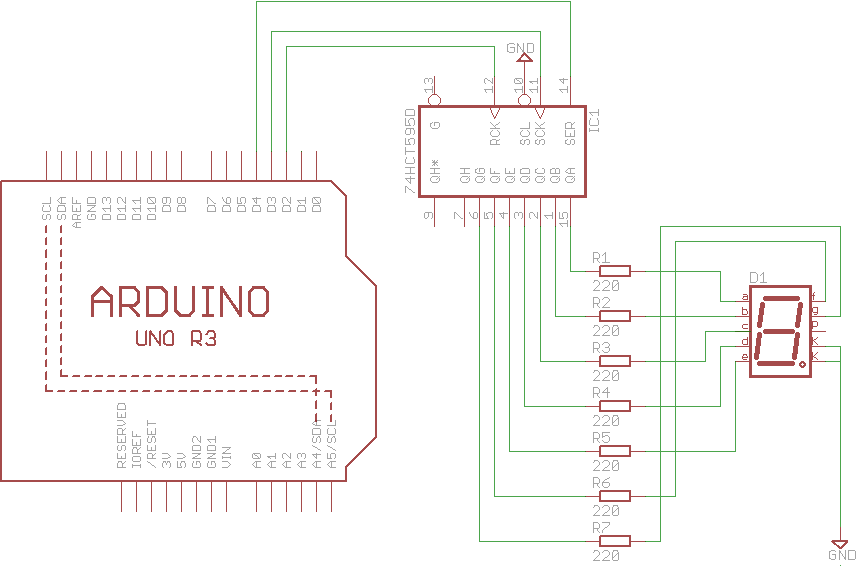
\includegraphics[scale=0.85]{img/Ard-shift}

\caption{Arduino with a shift register and a 7-segments display (schematic) \label{fig:ard-shift}}

\end{figure}

The schematic is not complete but can show the advantages of the use of a shift register to hold 
the data for the display, and shift out the data to the next one when requested. 
The next step is to connect together more shift registers and more displays in a cascade 
connection, which can be extended without the need of many digital outputs from the CPU.
Figure \ref{fig:ard-4xshift} shows an example of this connection type; this is exactly the configuration 
where this library comes in real help.

%
\begin{figure}[H]
\centering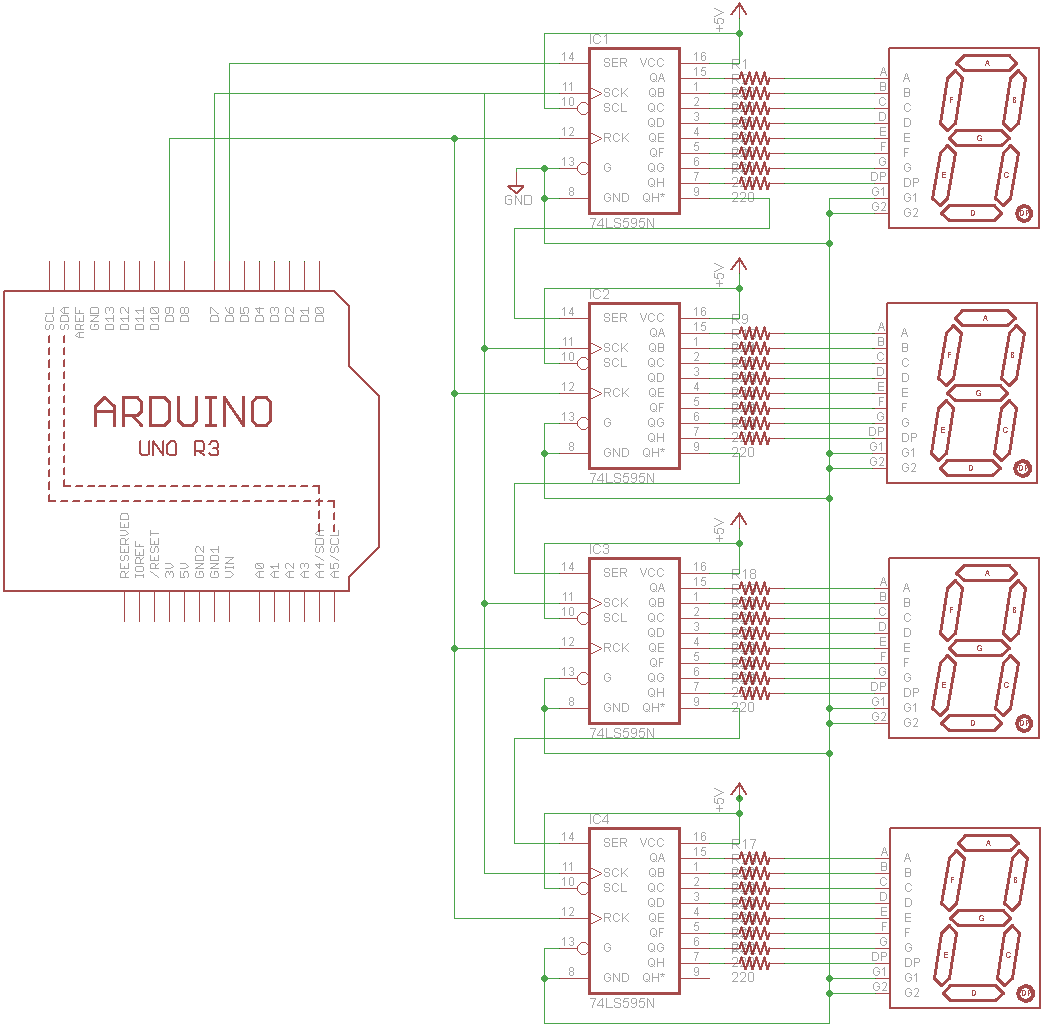
\includegraphics[scale=0.75]{img/4x-shift-reg}

\caption{Arduino with 4 shift registers and 4 7-segments display (schematic) \label{fig:ard-4xshift}}

\end{figure}



\subsection{What is this library for?}\label{subsec:what does}

Let's suppose you have many displays, each of them with its register, like in figure \ref{fig:ard-4xshift},
and you have to shows different variables on different displays, but some of this variables have one 
digit, other have two or three digits and so on. You could make a program (sketch) for Arduino to 
manage this situation, but this library is a more convenient way.
The design is based on the \textbf{display group} concept: this is a set of semantically linked displays, 
like two displays which represent the two digits of the \emph{same} number (or value).
%
\begin{figure}[htb]
\centering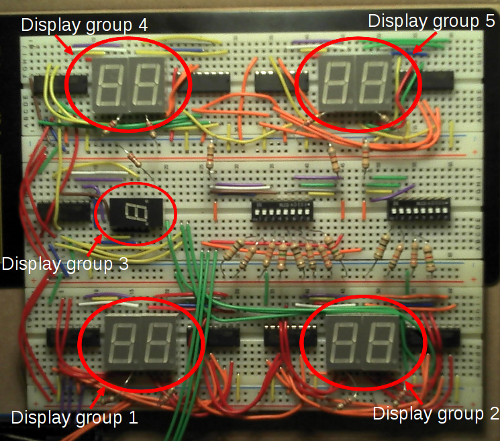
\includegraphics[scale=0.7]{img/Dis-group}

\caption{Breadboard with 5 display group \label{fig:dis-group}}

\end{figure}

In figure \ref{fig:dis-group} there are many display group, each with a different role. The library is 
able to keep the informations regarding each display group and update all the display group when some 
of the values has changed. In addition every group can pad the unused display with zeros automatically, 
depending of the number of digit currently used by the represented variable.

This allows a easy management of many displays without worries about the update and configuration 
in the main program.
Now let's dive more deeply into details!


\section{Library classes}\label{sec:lib-classes}


\subsection{Display}

This class represent a single 7-segments display and is a low level class that uses some Arduino 
primitives to change the state of hardware digital output, and update the shift register associated 
with the display.  
%
\begin{lstlisting}[label=lis:dis-class,caption=Display class]
class Display {
public:

  Display();

  Display(const byte digits[]);

  virtual ~Display();

  void update(byte digit) const;

  void turnOff() const;

  byte getBitOrder() const;

  void setBitOrder(byte bitOrder);

private:

  byte _digits[10]; 
  byte _bitOrder;   
};
\end{lstlisting}

The \code{\_digits[]} array holds the representation for every digits, from 0 to 9: the \emph{i-th} 
component of the array indicates which segment will be turned on when the display will show the digit 
\emph{i}.
The main method is \code{update()}, shown in listing \ref{lis:dis-update}:
%
\begin{lstlisting}[label=lis:dis-update,caption=Display update method]
void Display::update(byte digit) {
  byte v = _digits[digit];

  for (byte bitMask = 128; bitMask > 0; bitMask >>= 1) {
    digitalWrite(DisplayManager::clockPin, LOW);
    digitalWrite(DisplayManager::dataPin, v & bitMask ? HIGH : LOW);
    digitalWrite(DisplayManager::clockPin, HIGH);
  }
}
\end{lstlisting}

This method takes a digit [0-9] and sends to the shift register the correct sequence of bit, using 
a data pin and a clock pin to shift out the bits. The method uses the C/C++ bit-twiddling technique, but 
there are other ways of doing the same thing: the Arduino site has a good language reference on 
\emph{shiftOut} \footnote{\url{http://www.arduino.cc/en/Reference/ShiftOut}} and also a tutorial on 
using the 74HC595s \footnote{\url{http://www.arduino.cc/en/Tutorial/ShiftOut}}. The problem with 
\emph{shiftOut} is that you can't put some delay between data pin update and the rising edge of the 
clock pin, and this in some cases can lead to wrong communication.
Every time this method is called, 8 bits are shifted out on the data pin, and these will fill 
the shift register connected to the 7-segments display. Once the last bit has been transfered the 
register will light up the correct segments (this behavior depends on the shift register begin used).

Another useful method is \code{turnOff()} which simply shifts 8 low bits (zeros) when called. With this 
method a display can be turned off from the software without disconnect the power supply.
This will be used in the scoreboard project, to setup a volleyball configuration.


\subsection{DisplayGroup}

This class represent the core of the library and manages many \code{Display} object to show the 
correct digit in every position. This is useful when a multi-digit number has to be shown: this class 
does the hard work of splitting every digits and send it to the correct display. Each of \code{Display} 
object correspond to a real 7-segments display.
%
\begin{lstlisting}[label=lis:dis-group-class,caption=DisplayGroup class]
class DisplayGroup {
public:

  DisplayGroup(byte nDisplay, byte id, uint16_t * value, const byte digits[]);

  virtual ~DisplayGroup();

  int update() const;

  byte getId() const;

  byte getDisplayNumber() const;

  byte getBitOrder() const;

  void setBitOrder(byte bitOrder);

  void setEnabled(boolean enabled);

private:

  std::vector<Display> _displays; 
  byte _id;                       
  uint16_t * _value;              
  byte _nDisplay;                 
  byte _bitOrder;                 
  boolean _enabled;               
};
\end{lstlisting}

The \code{DisplayGroup} class holds a vector of \code{Display} objects and the address of the 
variable to be represented on the displays (\code{\_value}). 
The constructor is shows in listing \ref{lis:group-cons}:
%
\begin{lstlisting}[label=lis:group-cons,caption=DisplayGroup class constructor]
DisplayGroup::DisplayGroup(byte nDisplay, byte id, uint16_t * value, const byte digits[]) :
    _id(id), _nDisplay(nDisplay) {

  Display dis(digits);
  _displays.assign(nDisplay, dis);

  _enabled = true;
  _value = value;
}
\end{lstlisting}
%
It is also possible to change the encoding of the display per group, so if the displays in 
the application have different encoding the library can be configured accordingly.
This can be done by passing the desired \code{digits} array.
The \code{\_enabled} property describes whether the DisplayGroup is active or not: in the latter 
case all the inner Display objects will be turned off through the special method \code{turnOff()}.

The value of the memory location pointed to by \code{\_value} is checked when the update 
method is called. The update process is described in \ref{subsec:group-update}.



\subsubsection{Group update} \label{subsec:group-update}

The \code{update} method take the content of the pointer \code{\_value} and elaborates the 
number with subsequent division by 10. Considering the quotient and the remainder of these 
division, the class is able to determine the number of digits, and which digits goes to the 
i-th display. The method takes also care of zero padding and filling when the value has less 
digits than the number of display in the group.
%
\begin{lstlisting}[label=lis:group-update,caption=DisplayGroup update method]
int DisplayGroup::update() const {
  if (_nDisplay == 0) {
    return -1;
  }

  // Turn off al the displays
  if (!_enabled) {
    std::vector<Display>::const_iterator beg = _displays.begin();
    std::vector<Display>::const_iterator end = _displays.end();

    for (; beg != end; ++beg) {
      (*beg).turnOff();
    }

    return 0;
  }

  if (!_value) {
    return -2;
  }

  // Quotient
  uint16_t quot = *(_value) / 10;
  uint16_t tempV = quot;
  // Division counter
  byte divCount = 1;
  boolean filled = false;

  // Update the first display
  _displays[0].update(*(_value) % 10);

  // Look for zero filling in heading when *(_value) is < 10
  if (quot == 0) {
    for (byte i = 1; i < _nDisplay; ++i) {
      _displays[i].update(0);
    }
    filled = true;
  }

  // Count up division by 10 updates display with the remainder
  while (quot != 0 && divCount < _nDisplay) {
    quot = tempV / 10;

    _displays[divCount].update(tempV % 10);
    divCount++;

    tempV = quot;
  }

  // Return -3 if the number cannot be displayed with the number of displays in
  // the group
  if (divCount == _nDisplay && quot != 0) {
    return -3;
  } else if (divCount < _nDisplay && !filled) {
    // Look for zero filling in heading when *(_value) is > 10
    for (byte i = divCount; i < _nDisplay; ++i) {
      _displays[i].update(0);
    }
  }

  return 0;
}
\end{lstlisting}

Every time a digit is ready the \code{Display.update()} method gets called with the correct value, 
shifting out all the required bits to the digital connections.


\subsection{DisplayManager}

This class is the interface between the library and the main code. 
%                                       
\begin{lstlisting}[label=lis:display-manager,caption=DisplayManager class]
class DisplayManager {
public:

  static const byte DEF_DIGITS[10]; 
  static const byte DEF_ORDER;      

  static byte dataPin;          
  static byte clockPin;         
  static byte outputEnablePin;  


  DisplayManager(byte dataP, byte clockP, byte outputEnableP);

  virtual ~DisplayManager();

  void addGroup(byte id, byte nDisplay,uint16_t * value);

  void addGroup(byte id, byte nDisplay, uint16_t * value, const byte digits[], byte sizeOfDigits);

  void insertGroup(byte id, byte nDisplay, byte index, uint16_t * value);

  void insertGroup(byte id, byte nDisplay, byte index, uint16_t * value, const byte digits[], byte sizeOfDigits);

  void replaceGroup(byte id, byte nDisplay, uint16_t * value);

  void replaceGroup(byte id, byte nDisplay, uint16_t * value, const byte digits[], byte sizeOfDigits);

  void removeGroup(byte id);

  void clearGroups();

  void enableGroup(byte id, boolean enable);

  uint16_t updateAll() const;

  void setBitOrder(byte id, byte order);

  String printGroups() const;

private:

  std::deque<DisplayGroup> _groups;

};
\end{lstlisting}



This class hold its own vector of \code{DisplayGroup} objects, which can be created and inserted at 
runtime. Every group has a name, a number of contained displays and an \code{id} property; this is 
used to keep a unique reference to each group, and to insert or remove the group with the specified
id from the manager.
The method \code{addGroup()} construct a DisplayGroup object and adds it at the end of the manager's 
vector. The methods \code{replaceGroup()} and \code{insertGroup()} have and \code{index} parameter: 
this parameter specify the actual index of the new DisplayGroup that will be inserted in the vector.

The most important method is \code{updateAll()}:
%                                       
\begin{lstlisting}[label=lis:display-manager-update, caption=DisplayManager update method]
uint16_t DisplayManager::updateAll() {
  uint16_t ret = 0, idx = 0;

  digitalWrite(outputEnablePin, HIGH);

  // Reverse iteration to account for shift register serial update order
  std::deque<DisplayGroup>::reverse_iterator beg = _groups.rbegin();
  std::deque<DisplayGroup>::reverse_iterator end = _groups.rend();

  for (idx = 0; beg != end; ++beg, ++idx) {
    if ((*beg).update() != 0) {
      ret = idx;
    }
  }

  digitalWrite(outputEnablePin, LOW);

  return ret;
}
\end{lstlisting}

The method iterates over the vector to call the \code{update()} method on every \code{DisplayGroup} 
object. The iteration is done in reverse order because the first data output on the bus will go 
on the last 7-segments displays in the queue. So this displays must be the first to be updated.

During this procedure the output enable pin on the shift registers are disabled, to ensure there are 
no glitches on the LEDs.



\section{Architecture}\label{sec:arc}

The library has been developed following a design patter similar to the Observer design patter from
GoF. The patter I used is slightly different, with some simplification, to avoid too much code 
overhead in th CPU, which has only 32KB of flash memory available to store the program. The patter 
is described in section \ref{subsec:design}.

The main data structure, holding the information for all the displays, is made of standard STL vectors, 
which provides fast iteration and preserve order. This is described in section \ref{subsec:stl}.



\subsection{Design pattern}\label{subsec:design}

The standard GoF Observer Design Pattern \footnote{\url{http://en.wikipedia.org/wiki/Observer_pattern}} 
was made to define a one-to-many dependency between objects so that when one object changes state, all 
its dependents are notified and updated automatically. This behavior is close to what I needed to update 
all the displays when some related values changes, so I needed to modify the standard patter and use a 
specialized version.

%
\begin{figure}[htb]
\centering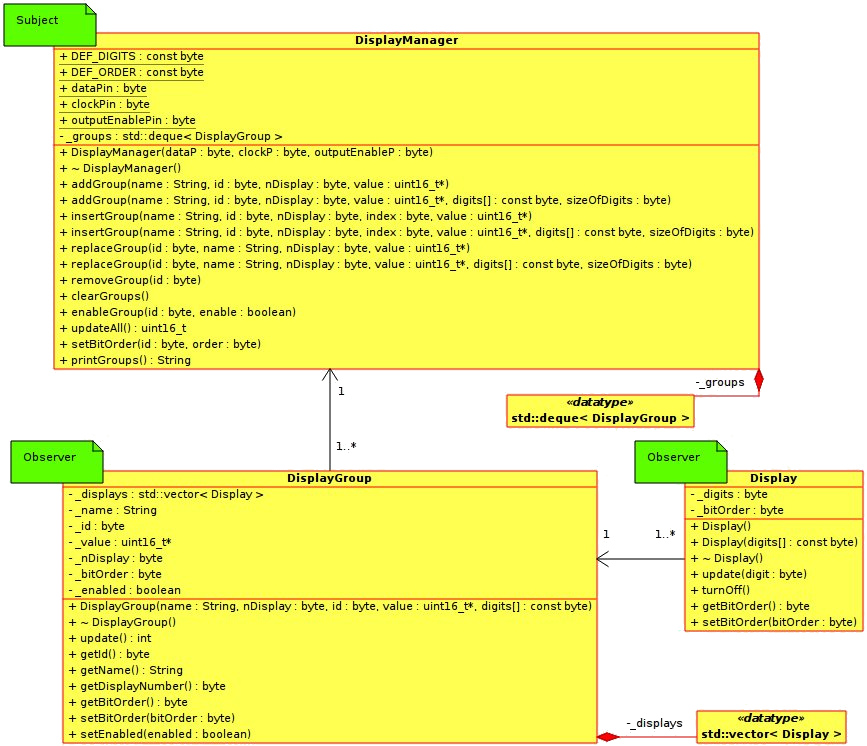
\includegraphics[scale=0.65]{img/UML}

\caption{UML diagram for DisplayGroup library \label{fig:uml}}

\end{figure}

In this version there is only one subject (\code{DisplayManager}), which notify all its observer with their 
\code{update()} methods, running through all the \code{DisplayGroup}. These objects are subject on their own, 
and they notify all their observer, the \code{Display} objects, through their method \code{Display.update()}. 

The figure \ref{fig:uml} shows the UML diagram with the relationship between the elements of the pattern.
This patter make possible a very simple interaction between the main code and the library: an example will be 
given in section \ref{sec:test}.


\subsection{STL containers}\label{subsec:stl}

The C++ Standard Template Library is commonly used in all kind of application, but in this case it has been 
compiled and applied to a basic 8-bit microcontroller CPU. The inclusion procedure is pretty straightforward, 
but in the INSTALL file you can find some links to download the library for Arduino and compile a sketch in 
your own environment (Thanks to Andy Brown 
\footnote{\url{http://andybrown.me.uk/wk/2011/01/15/the-standard-template-library-stl-for-avr-with-c-streams/}}).

The main data structure used in the DisplayGroup library is made of deques, because they provide fast random 
access and iteration, and preserve the order of the elements. This last property is really important to 
update all the displays in the correct order!
The possibility to iterate backwards in the container is another property which made the update code much 
easier (listing \ref{lis:display-manager-update}). Vectors could have been used for the same reasons, but the 
automatic capacity management creates an out of memory problem on a platform like the Arduino Uno. Too much 
memory is used \emph{in advance} already after the second insertion of an element: this 
happens because \textquotedblleft vector containers may allocate some extra storage to accommodate for possible 
growth, and thus the container may have an actual capacity greater than the storage strictly needed to contain 
its elements (i.e., its size) \textquotedblright \footnote{\url{http://www.cplusplus.com/reference/vector/vector/}}.

The \code{DisplayGroup} class still uses vectors, because the constructor calls the \code{assign()} method which 
causes an automatic reallocation of the allocated storage space if -and only if- the new vector size surpasses the 
current vector capacity. In this case the size \emph{and} the capacity remain equal so the allocated memory 
does not grow dramatically at runtime.

In the \code{DisplayManager} class some STL algorithms are used: find\_if, replace\_if. All those 
algorithms use a binary predicate that is generated from a unary predicate following the C++ \emph{functional} 
paradigm.
The STL provides a template function for this conversion that takes a binary predicate and turns it into a 
unary predicate. The compositor function is called \code{bind2nd()} (that is, bind the second argument into 
the binary predicate to produce a unary predicate), so the goal is to produce what the STL calls an 
\emph{Adaptable Binary Predicate}.
The predicate is shown in listing \ref{lis:display-manager-predicate}:

%                                       
\begin{lstlisting}[label=lis:display-manager-predicate, caption=DisplayManager: STL Adaptable Binary Predicate 
for find and replace algorithms]
struct GroupId: public std::binary_function<DisplayGroup, byte, bool> {
  bool operator () (const DisplayGroup &gr, const byte &id) const {
    return gr.getId() == id;
  }
};

if (std::find_if(_groups.begin(), _groups.end(), std::bind2nd(GroupId(), id)) == _groups.end()) {
// Group with id not found
...
}
\end{lstlisting}

The data structure can handle a general set of DisplayGroup (and Displays), and is accessed and 
modified with the previously described STL algorithms and vectors API:

%
\begin{figure}[htb]
\centering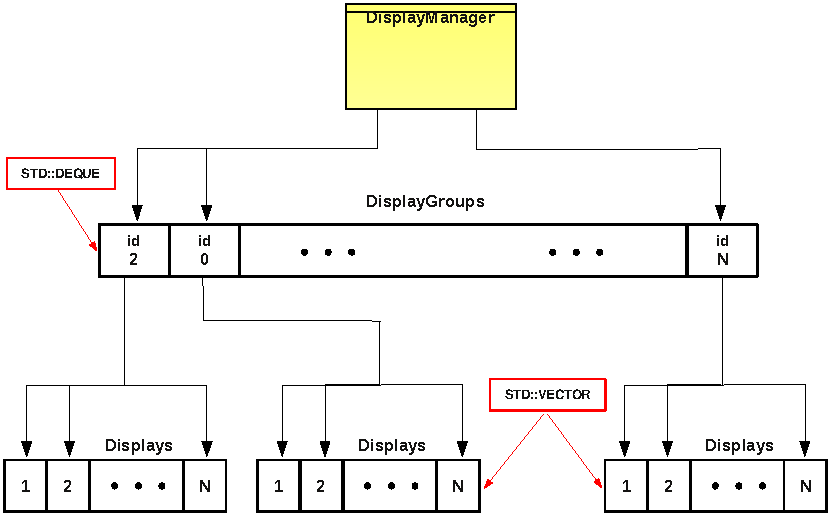
\includegraphics[scale=0.85]{img/Vectors}

\caption{Vectors data structure, composed by a DisplayManager, many DisplayGroup, and many Display for each 
group  \label{fig:vectors}}

\end{figure}

Figure \ref{fig:vectors} shows a schematic representation of the data structure: this allows the creation of 
multiple display group in the application and for each group is possible to assign as many display as needed.
The application has been tested with few display, so it can happen, with an high number of display, that the 
user need to take into account some transmission delay during the shift out, and also the \underline{limited} 
quantity of RAM memory on the Arduino UNO board can be a problem.

\pagebreak

\section{Test}\label{sec:test}

The library has been tested with both a breadboard circuit and a real use circuit, with different hardware.
The test code \footnote{\url{http://display-group.googlecode.com/svn/trunk/DisplayGroupTest}} creates two group 
with two displays each, and demonstrates how to link some variables and update all the displays, even with 
different encodings among groups.
%                                       
\begin{lstlisting}[label=lis:display-manager-create, caption=DisplayManager: constructor call]
  // Display manager to manage all the connected display, organized as groups.
  DisplayGroup::DisplayManager disManager(gPinData, gPinClock, gOutputEnable);
\end{lstlisting}

The DisplayManager API can be used to insert some DisplayGroup object, and set some of their properties.
For example the \code{index} property should match the order of the display in the physical connection, 
starting from the one closest to Arduino.
%                                       
\begin{lstlisting}[label=lis:add-group, caption=DisplayManager: adding groups to the manager]
  // AddGroup parameters: name of the group, number of displays, index, 
  // address of the value, encoding, size of the encoding array
  disManager.addGroup(2, 0, &gNumberToDisplay2, gDigits7, sizeof(gDigits7));
  disManager.addGroup(2, 1, &gNumberToDisplay1, gDigits4, sizeof(gDigits4));
\end{lstlisting}

All the previous setting should be done in the \code{setup()} method in the Arduino sketch.
In the \code{loop()} the method \code{updateAll()} can be called to iterate over the collection 
of displays and shift out the data to the serial bus (SPI interface).
%                                       
\begin{lstlisting}[label=lis:display-manager-updateall, caption=DisplayManager: update all groups]
  disManager.updateAll();
  delay(1200);

  gNumberToDisplay1++;
  if (gNumberToDisplay1 == 100) {
    gNumberToDisplay1 = 0;
  }
  ...
\end{lstlisting}


The breadboard test has already been shown in figure \ref{fig:dis-group}, while the real application 
\footnote{\url{https://plus.google.com/photos/109652469005118520122/albums/5799213099932281809}} is shown 
in the next figure. 
The code \footnote{\url{http://display-group.googlecode.com/svn/trunk/ScoreBoard}} for the display 
management is very similar to the test one, except for some parts related to time management and user input.
%
\begin{figure}[H]
\centering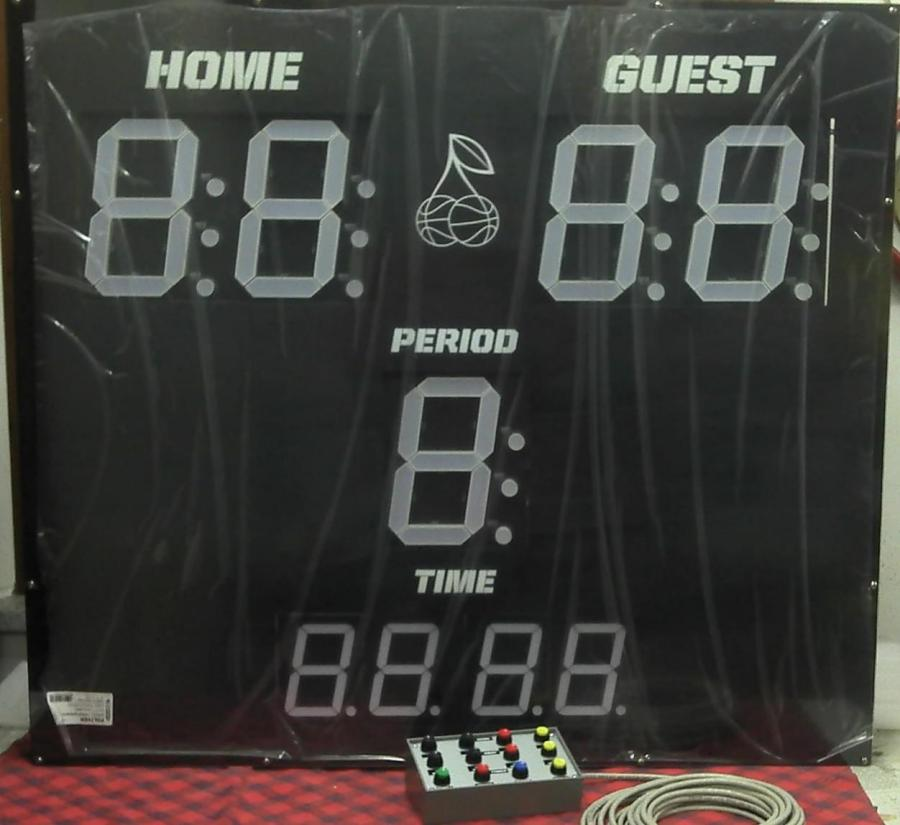
\includegraphics[scale=0.55]{img/ScoreBoard}

\caption{ScoreBoard application: realized for a local basketball team!!\label{fig:scoreboard}}

\end{figure}


\section{Future improvement}\label{sec:future}

The library is already working good for my needs but there are many improvements that could be done to
enhance the safeness of the code and to make available other features:

\begin{itemize}
 \item better management of Arduino UNO r3 small memory quantity (2 KB);
 \item partial code rewrite to avoid some design drawback: for example the need to pass a pointer to some 
       methods, which can be \code{NULL} at runtime;
 \item floating point support: to show floating numbers on the displays;
\end{itemize}

In particular when the application has more than 6-7 DisplayGroup the CPU can run out of memory (you can 
check the available RAM memory with the MemoryFree \footnote{\url{http://playground.arduino.cc/Code/AvailableMemory}} 
library). In this case the platform can be completely stuck and is a not so easy to debug situation!

\end{document}
